% Figure from MATH 591 notes, section 71 (after the board). Compile with the notes preamble.
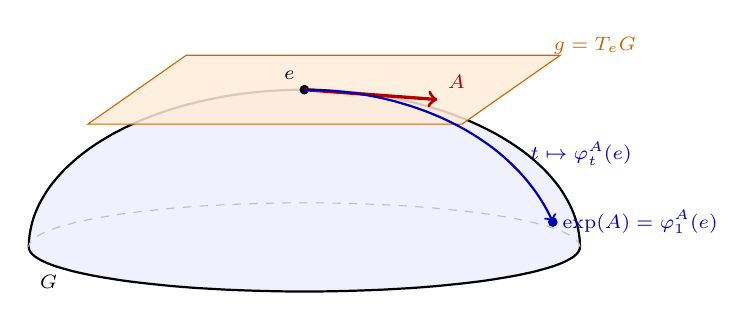
\begin{tikzpicture}[scale=1.25]
\fill[blue!6] plot[smooth] coordinates {(2.800,0.000) (2.798,0.064) (2.791,0.127) (2.780,0.190) (2.765,0.253) (2.745,0.316) (2.721,0.378) (2.692,0.440) (2.659,0.500) (2.623,0.560) (2.582,0.620) (2.536,0.678) (2.487,0.735) (2.434,0.791) (2.377,0.845) (2.316,0.899) (2.252,0.951) (2.184,1.001) (2.113,1.050) (2.038,1.097) (1.960,1.143) (1.879,1.186) (1.795,1.228) (1.708,1.268) (1.619,1.306) (1.527,1.341) (1.432,1.375) (1.335,1.406) (1.236,1.436) (1.135,1.463) (1.033,1.487) (0.929,1.509) (0.823,1.529) (0.716,1.547) (0.608,1.562) (0.498,1.574) (0.388,1.585) (0.278,1.592) (0.167,1.597) (0.056,1.600) (-0.056,1.600) (-0.167,1.597) (-0.278,1.592) (-0.388,1.585) (-0.498,1.574) (-0.608,1.562) (-0.716,1.547) (-0.823,1.529) (-0.929,1.509) (-1.033,1.487) (-1.135,1.463) (-1.236,1.436) (-1.335,1.406) (-1.432,1.375) (-1.527,1.341) (-1.619,1.306) (-1.708,1.268) (-1.795,1.228) (-1.879,1.186) (-1.960,1.143) (-2.038,1.097) (-2.113,1.050) (-2.184,1.001) (-2.252,0.951) (-2.316,0.899) (-2.377,0.845) (-2.434,0.791) (-2.487,0.735) (-2.536,0.678) (-2.582,0.620) (-2.623,0.560) (-2.659,0.500) (-2.692,0.440) (-2.721,0.378) (-2.745,0.316) (-2.765,0.253) (-2.780,0.190) (-2.791,0.127) (-2.798,0.064) (-2.800,0.000)} -- plot[smooth] coordinates {(-2.800,0.000) (-2.796,-0.024) (-2.784,-0.048) (-2.764,-0.072) (-2.737,-0.095) (-2.701,-0.118) (-2.658,-0.141) (-2.608,-0.164) (-2.550,-0.186) (-2.485,-0.207) (-2.412,-0.228) (-2.333,-0.249) (-2.248,-0.268) (-2.156,-0.287) (-2.057,-0.305) (-1.953,-0.322) (-1.844,-0.339) (-1.729,-0.354) (-1.609,-0.368) (-1.485,-0.381) (-1.357,-0.394) (-1.224,-0.405) (-1.089,-0.415) (-0.950,-0.423) (-0.808,-0.431) (-0.665,-0.437) (-0.519,-0.442) (-0.372,-0.446) (-0.223,-0.449) (-0.075,-0.450) (0.075,-0.450) (0.223,-0.449) (0.372,-0.446) (0.519,-0.442) (0.665,-0.437) (0.808,-0.431) (0.950,-0.423) (1.089,-0.415) (1.224,-0.405) (1.357,-0.394) (1.485,-0.381) (1.609,-0.368) (1.729,-0.354) (1.844,-0.339) (1.953,-0.322) (2.057,-0.305) (2.156,-0.287) (2.248,-0.268) (2.333,-0.249) (2.412,-0.228) (2.485,-0.207) (2.550,-0.186) (2.608,-0.164) (2.658,-0.141) (2.701,-0.118) (2.737,-0.095) (2.764,-0.072) (2.784,-0.048) (2.796,-0.024) (2.800,-0.000)} -- cycle;
\draw[thick] plot[smooth] coordinates {(2.800,0.000) (2.798,0.064) (2.791,0.127) (2.780,0.190) (2.765,0.253) (2.745,0.316) (2.721,0.378) (2.692,0.440) (2.659,0.500) (2.623,0.560) (2.582,0.620) (2.536,0.678) (2.487,0.735) (2.434,0.791) (2.377,0.845) (2.316,0.899) (2.252,0.951) (2.184,1.001) (2.113,1.050) (2.038,1.097) (1.960,1.143) (1.879,1.186) (1.795,1.228) (1.708,1.268) (1.619,1.306) (1.527,1.341) (1.432,1.375) (1.335,1.406) (1.236,1.436) (1.135,1.463) (1.033,1.487) (0.929,1.509) (0.823,1.529) (0.716,1.547) (0.608,1.562) (0.498,1.574) (0.388,1.585) (0.278,1.592) (0.167,1.597) (0.056,1.600) (-0.056,1.600) (-0.167,1.597) (-0.278,1.592) (-0.388,1.585) (-0.498,1.574) (-0.608,1.562) (-0.716,1.547) (-0.823,1.529) (-0.929,1.509) (-1.033,1.487) (-1.135,1.463) (-1.236,1.436) (-1.335,1.406) (-1.432,1.375) (-1.527,1.341) (-1.619,1.306) (-1.708,1.268) (-1.795,1.228) (-1.879,1.186) (-1.960,1.143) (-2.038,1.097) (-2.113,1.050) (-2.184,1.001) (-2.252,0.951) (-2.316,0.899) (-2.377,0.845) (-2.434,0.791) (-2.487,0.735) (-2.536,0.678) (-2.582,0.620) (-2.623,0.560) (-2.659,0.500) (-2.692,0.440) (-2.721,0.378) (-2.745,0.316) (-2.765,0.253) (-2.780,0.190) (-2.791,0.127) (-2.798,0.064) (-2.800,0.000)};
\draw[thick] plot[smooth] coordinates {(-2.800,0.000) (-2.796,-0.024) (-2.784,-0.048) (-2.764,-0.072) (-2.737,-0.095) (-2.701,-0.118) (-2.658,-0.141) (-2.608,-0.164) (-2.550,-0.186) (-2.485,-0.207) (-2.412,-0.228) (-2.333,-0.249) (-2.248,-0.268) (-2.156,-0.287) (-2.057,-0.305) (-1.953,-0.322) (-1.844,-0.339) (-1.729,-0.354) (-1.609,-0.368) (-1.485,-0.381) (-1.357,-0.394) (-1.224,-0.405) (-1.089,-0.415) (-0.950,-0.423) (-0.808,-0.431) (-0.665,-0.437) (-0.519,-0.442) (-0.372,-0.446) (-0.223,-0.449) (-0.075,-0.450) (0.075,-0.450) (0.223,-0.449) (0.372,-0.446) (0.519,-0.442) (0.665,-0.437) (0.808,-0.431) (0.950,-0.423) (1.089,-0.415) (1.224,-0.405) (1.357,-0.394) (1.485,-0.381) (1.609,-0.368) (1.729,-0.354) (1.844,-0.339) (1.953,-0.322) (2.057,-0.305) (2.156,-0.287) (2.248,-0.268) (2.333,-0.249) (2.412,-0.228) (2.485,-0.207) (2.550,-0.186) (2.608,-0.164) (2.658,-0.141) (2.701,-0.118) (2.737,-0.095) (2.764,-0.072) (2.784,-0.048) (2.796,-0.024) (2.800,-0.000)}; \draw[gray!50, dashed] plot[smooth] coordinates {(2.800,0.000) (2.796,0.024) (2.784,0.048) (2.764,0.072) (2.737,0.095) (2.701,0.118) (2.658,0.141) (2.608,0.164) (2.550,0.186) (2.485,0.207) (2.412,0.228) (2.333,0.249) (2.248,0.268) (2.156,0.287) (2.057,0.305) (1.953,0.322) (1.844,0.339) (1.729,0.354) (1.609,0.368) (1.485,0.381) (1.357,0.394) (1.224,0.405) (1.089,0.415) (0.950,0.423) (0.808,0.431) (0.665,0.437) (0.519,0.442) (0.372,0.446) (0.223,0.449) (0.075,0.450) (-0.075,0.450) (-0.223,0.449) (-0.372,0.446) (-0.519,0.442) (-0.665,0.437) (-0.808,0.431) (-0.950,0.423) (-1.089,0.415) (-1.224,0.405) (-1.357,0.394) (-1.485,0.381) (-1.609,0.368) (-1.729,0.354) (-1.844,0.339) (-1.953,0.322) (-2.057,0.305) (-2.156,0.287) (-2.248,0.268) (-2.333,0.249) (-2.412,0.228) (-2.485,0.207) (-2.550,0.186) (-2.608,0.164) (-2.658,0.141) (-2.701,0.118) (-2.737,0.095) (-2.764,0.072) (-2.784,0.048) (-2.796,0.024) (-2.800,0.000)};
\fill[orange!15, opacity=0.85] (-2.2,1.25) -- (1.6,1.25) -- (2.6,1.95) -- (-1.2,1.95) -- cycle;
\draw[orange!80!black] (-2.2,1.25) -- (1.6,1.25) -- (2.6,1.95) -- (-1.2,1.95) -- cycle;
\node[orange!80!black, font=\scriptsize] at (2.95,2.05) {$\mathfrak{g} = T_eG$};
\fill (0,1.6) circle (1.4pt) node[above left, font=\scriptsize] {$e$};
\draw[->, very thick, red!70!black] (0,1.6) -- (1.35,1.5) node[above right, font=\scriptsize] {$A$};
\draw[blue!70!black, thick, ->] plot[smooth] coordinates {(0.000,1.600) (0.085,1.599) (0.170,1.596) (0.255,1.591) (0.340,1.584) (0.424,1.575) (0.508,1.565) (0.592,1.552) (0.675,1.537) (0.757,1.521) (0.838,1.502) (0.919,1.482) (0.998,1.459) (1.077,1.435) (1.154,1.409) (1.230,1.382) (1.305,1.352) (1.379,1.321) (1.451,1.288) (1.522,1.253) (1.591,1.217) (1.658,1.179) (1.724,1.139) (1.788,1.098) (1.850,1.055) (1.911,1.011) (1.969,0.965) (2.025,0.918) (2.079,0.869) (2.131,0.819) (2.181,0.768) (2.229,0.715) (2.274,0.661) (2.317,0.606) (2.358,0.550) (2.396,0.493) (2.432,0.435) (2.465,0.376) (2.496,0.316) (2.524,0.255)};
\fill[blue!70!black] (2.524,0.255) circle (1.4pt) node[right, font=\scriptsize] {$\exp(A) = \varphi^A_1(e)$};
\node[blue!70!black, font=\scriptsize, anchor=west] at (2.2,0.95) {$t \mapsto \varphi^A_t(e)$};
\node[font=\scriptsize] at (-2.6,-0.35) {$G$};
\end{tikzpicture}
